\documentclass{article}
\usepackage{graphicx}
\usepackage{subcaption}
\usepackage[
    top = 1cm,
    left=2cm,
    right=2cm,
    bottom = 1cm
]{geometry}
\usepackage{float}
\usepackage{dirtree}
\usepackage{amsmath}
\usepackage[portuguese, ruled, linesnumbered]{algorithm2e}

\title{Projeto 02: Aprendizado por Reforço\\ \large Decisões Financeiras em Portfólio Simplificado}
\author{
  \small
  Bruno Amaral Salles (281129) \textbullet{} Rodrigo Banin Ferraz de Camargo (238257) \\
  \small
    Caio Lima Albulquerque (288808) \textbullet{} João Pedro Bonatti (237575) \textbullet{} Ricardo Andrade Oliveira Bello (247326)
  \date{\small\today}
}
\begin{document}
\maketitle

\section{Introdução - Modelagem do Problema}
Este projeto trata do desenvolvimento de um agente treinado por Aprendizado por Reforço para a tomada de decisões financeiras sequenciais. O ambiente simula um portfólio simplificado de investimentos, no qual o agente interage com dados históricos reais de ações da Amazon. O desafio é aprender uma política que maximize o retorno financeiro acumulado ao longo do tempo, operando sob a incerteza das variações de preço. Para a aplicação dos algoritmos de aprendizado, o problema foi formalizado como um Processo de Decisão de Markov (MDP), definido pela tupla $(S, A, T, R)$.

\subsection{Representação do Estado ($S$)}
O estado $S$ constitui uma representação discretizada da condição momentânea do mercado e é representado por uma tupla de quatro variáveis binárias: $S = (p, \upsilon, \mu, \rho)$:
\begin{itemize}
    \item \textbf{Posição ($p$):} Indica se o agente possui o ativo ($1$) ou não ($0$).

    \item \textbf{Volatilidade ($\upsilon$):} Indica a estabilidade do mercado ($1$ se o desvio padrão dos últimos 10 dias for superior a $0.015$, caso contrário $0$).

    \item \textbf{MACD - Convergência/Divergência de médias móveis ($\mu$):} Mede a tendência e o impulso do preço de um ativo com base nas Médias Móveis Longas (26 dias) e Curtas (12 dias).
    \begin{equation}
        \text{Linha MACD} = \text{MME}_{12} - \text{MME}_{26}
    \end{equation}
    Por fim, calcula-se a diferença entre MACD e a média móvel do MACD de 9 dias. O estado é 1 para o caso em que o MACD é positivo e, caso contrário, 0.
    \begin{equation}
        \text{MACD} = \text{Linha MACD} - \text{Linha de Sinal}
    \end{equation}
    \item \textbf{RSI - Índice de Força Relativa ($\rho$):} Mede a velocidade e a mudança dos movimentos de preço. O cálculo inicia-se pela determinação da Força Relativa ($RS$):
    \begin{equation}
        RS = \frac{\text{Ganho Médio}}{\text{Perda Média}}
    \end{equation}
    Em seguida, esse valor é transformado para uma escala oscilatória entre 0 e 100:
    \begin{equation}
        RSI = 100 - \left( \frac{100}{1 + RS} \right)
    \end{equation}
\end{itemize}

\subsection{Ações ($A$)}
O agente possui um espaço de ações $A$ discreto referente às operações do mercado financeiro. A cada avanço de tempo, o agente pode escolher $a \in \{-1, 0, 1\}$, onde:
\begin{itemize}
    \item \textbf{Comprar ($1$):} O agente altera sua posição para $1$, caso não esteja posicionado.
    \item \textbf{Vender ($-1$):} O agente liquida sua posição, alterando-a para $0$.
    \item \textbf{Manter ($0$):} O agente não realiza operações, mantendo a posição inalterada.
\end{itemize}

\subsection{Dinâmica do Ambiente ($T$)}
A transição entre estados $T(s, a, s')$ ocorre de forma sequencial seguindo os dados históricos do dataset utilizado. A cada ação $a$ realizada em $t$, o ambiente avança para $t+1$ e gera o novo estado $s'$ a partir do cálculo dos indicadores citados anteriormente. Embora os dados sejam históricos, a incerteza para o agente reside na impossibilidade de prever deterministicamente a próxima variação de preço apenas com os indicadores discretos atuais.

\subsection{Função de Reward ($R$)}
O sinal de recompensa $R(s, a, s')$ é calculado com base no preço de fechamento atual $P_t$ e no preço do dia anterior $P_{t-1}$:
\begin{equation}
    R_t = \left( \ln\left(\frac{P_t}{P_{t-1}}\right) \times p \right) - c
\end{equation}
Por fim, $p$ é a posição do agente no instante da transição e $c$ representa o custo de transação, fixado em $0.01$ sempre que ocorre uma troca de posição (compra ou venda). Esse custo penaliza movimentações excessivas e incentiva a busca por tendências de lucro consistentes.

\section{Equações de Bellman e Planejamento}
Com o objetivo de definir uma \textit{baseline} para o agente de aprendizado, foi implementado o algoritmo de \textit{Value Iteration}, uma técnica clássica de planejamento baseada em Programação Dinâmica. Diferente dos métodos de aprendizado por diferença temporal, ele necessita do conhecimento prévio da dinâmica do ambiente — isto é, das probabilidades de transição $T(s, a, s')$ e da função de recompensa esperada $R(s, a, s')$.

\subsection{Modelo de Transição Empírico}
Como o mercado financeiro (simulado pelo \texttt{StockMarketEnv}) não fornece um modelo de transição matemático fechado, o agente executa uma fase de "descoberta" antes do planejamento, simulando trajetórias ao longo dos dados históricos, mapeando empiricamente a probabilidade de transição entre o estado atual $s$ e o próximo estado $s'$, dado uma ação $a$, bem como a recompensa média obtida nessa transição. Esse modelo empírico possibilita a aplicação das Equações de Bellman.

\subsection{Atualização de Valor}
Com o modelo empírico construído, o algoritmo realiza "varreduras" (\textit{sweeps}) iterativas por todo o espaço de estados $S$. A cada iteração, o valor $V(s)$ de cada estado é atualizado aplicando a equação de otimalidade de Bellman:
\begin{equation}
    V(s) \leftarrow \max_{a} \sum_{s'} T(s,a,s') \left[ R(s,a,s') + \gamma V(s') \right]
\end{equation}
Esta atualização (conhecida como \textit{Bellman Backup}) calcula o valor máximo esperado para o estado $s$, ponderando as recompensas imediatas e o valor descontado ($\gamma$) dos possíveis estados futuros $s'$, de acordo com as probabilidades de transição $T$.

\subsection{Critério de Convergência}
Para garantir que o algoritmo não execute indefinidamente, é necessário definir um critério de parada. Por conta disso, um limiar de tolerância matemática denotado por $\theta = 10^{-4}$ foi adotado.

Durante uma varredura, o algoritmo monitora a maior alteração no valor de qualquer estado, calculada por $\Delta = \max_s |v - V(s)|$, onde $v$ é o valor do estado na iteração anterior. O \textit{Value Iteration} é interrompido quando $\Delta < \theta$. Em termos práticos, a convergência significa que as atualizações de valor se tornaram tão pequenas que a função de valor estabilizou e a política extraída a partir dela não sofrerá mais alterações significativas.

\subsection{Análise do Comportamento do Valor}
Ao longo das iterações, observou-se que o valor $V(s)$ dos estados associados a condições favoráveis de mercado cresceu rapidamente nas primeiras varreduras. O fator de desconto $\gamma$ determinou a velocidade de propagação desse valor para os estados predecessores. À medida que as iterações avançaram, os incrementos ($\Delta$) tornaram-se monotonicamente menores, confirmando a estabilidade da aproximação em direção ao valor ótimo, momento no qual a política ótima $\pi^*(s)$ pôde ser extraída de forma determinística:
\begin{equation}
    \pi^*(s) = \arg\max_{a} \sum_{s'} T(s,a,s') \left[ R(s,a,s') + \gamma V(s') \right]
\end{equation}

\section{Aprendizado por Diferença Temporal (TD Learning)}
Para que o agente aprenda a política ótima a partir da interação direta com o ambiente financeiro, sem depender de um modelo de transição prévio, foram implementados algoritmos de \textit{Temporal Difference} (TD) Control. O \textbf{protocolo experimental} adotado em todos os experimentos de TD obedeceu às exigências do enunciado: 5000 episódios fixos de treinamento, horizonte por episódio igual ao comprimento da série temporal de treino (\textit{full sweep}), inicialização padronizada da Q-table com zeros e instrumentação de recompensa, $\epsilon$ e número de \textit{steps} a cada episódio.

\subsection{Q-Learning}
O \textbf{Q-Learning} tem como objetivo permitir que o agente aprenda a política ótima iterativamente. Trata-se de um método \textit{model-free} e \textit{off-policy}, o que significa que ele atualiza a estimativa de valor assumindo que a próxima ação será sempre a melhor possível (ação gulosa), independentemente da política de exploração que o agente está seguindo no momento:
\begin{equation}
    Q(s,a) \leftarrow Q(s,a) + \alpha \left[ r + \gamma \max_{a'} Q(s',a') - Q(s,a) \right]
\end{equation}

\subsection{SARSA}
Para enriquecer a análise com fins de comparação e compreender o impacto da exploração durante o aprendizado, implementou-se de forma complementar o \textbf{SARSA} (State-Action-Reward-State-Action). Diferente do Q-Learning, trata-se de um método \textit{on-policy} que utiliza a estimativa da ação que efetivamente será tomada no próximo passo, refletindo de forma mais segura a política de exploração em curso:
\begin{equation}
    Q(s,a) \leftarrow Q(s,a) + \alpha \left[ r + \gamma Q(s',a') - Q(s,a) \right]
\end{equation}

\subsection{Estratégia de Exploração}
Para equilibrar a exploração de novas ações (visitar todo o espaço de estados) e a explotação do conhecimento já adquirido (maximizar o lucro), adotamos a estratégia $\epsilon$-greedy. O agente seleciona a melhor ação conhecida com probabilidade $1 - \epsilon$, e uma ação aleatória com probabilidade $\epsilon$. Avaliamos três diferentes estratégias de decaimento para ambos os algoritmos:
\begin{itemize}
    \item \textbf{Constante:} O valor de exploração permanece fixo durante todo o treinamento ($\epsilon = 0.2$).
    \item \textbf{Linear:} O $\epsilon$ é reduzido linearmente a cada episódio até alcançar um valor mínimo ($\epsilon_{start} = 1$ e $\epsilon_{end} = 0.05$).
    \item \textbf{Exponencial:} O $\epsilon$ decai exponencialmente a uma taxa constante ($\lambda = 0.9991$), reduzindo a exploração mais drasticamente no início.
\end{itemize}

\subsection{Inicialização dos Valores e Impacto dos Hiperparâmetros}
Antes do início do treinamento, todos os valores da matriz $Q(s,a)$ foram inicializados em zero. A convergência e o comportamento da política aprendida dependem diretamente de três hiperparâmetros fundamentais:
\begin{itemize}
    \item \textbf{Taxa de Aprendizado ($\alpha$):} Determina o peso da nova informação em relação ao conhecimento antigo. Valores altos de $\alpha$ fazem o agente aprender (e esquecer) rapidamente, o que pode causar oscilações no mercado financeiro. Valores muito baixos garantem estabilidade, mas exigem mais episódios para convergir.
    \item \textbf{Fator de Desconto ($\gamma$):} Define a importância das recompensas futuras. Um $\gamma$ próximo de 0 torna o agente impulsivo (focado apenas no lucro imediato), enquanto um $\gamma$ próximo de 1 faz o agente buscar estratégias de longo prazo. No mercado de ações, um $\gamma$ elevado é crucial para suportar a retenção (Hold) em vez de vender prematuramente.
    \item \textbf{Taxa de Exploração ($\epsilon$):} Regula o \textit{trade-off} entre exploração e explotação. Um $\epsilon$ mal ajustado pode impedir o agente de descobrir as melhores sequências de ações ou, inversamente, impedi-lo de usufruir da política ótima já descoberta.
\end{itemize}

\section{Avaliação Experimental}
A avaliação experimental foi conduzida com o objetivo de analisar o comportamento dos agentes sob diferentes configurações de hiperparâmetros, extraindo métricas de 5.000 episódios de treinamento. O foco da análise recaiu sobre a estabilidade, a eficiência de convergência e a capacidade de generalização das abordagens. As afirmações quantitativas desta seção são sustentadas pelas figuras apresentadas na Seção~\ref{sec:vis}.

\subsection{Comparação entre Estratégias de Exploração e Estabilidade}
A escolha da estratégia de decaimento da taxa de exploração ($\epsilon$) revelou-se um dos fatores mais determinantes para o sucesso do aprendizado, conforme evidenciado nas Figuras~\ref{fig:learning_curves} e \ref{fig:heatmap}. Agregando todas as configurações de $(\alpha, \gamma)$, a estratégia \textbf{Constante} ($\epsilon=0.2$) apresenta recompensa média nos últimos 100 episódios de $7.38$ (mediana $8.21$) — o ruído residual de 20\% de ações aleatórias impede a estabilização plena, gerando oscilações permanentes nas curvas correspondentes da Figura~\ref{fig:learning_curves}.

As estratégias \textbf{Exponencial} (média $7.58$, mediana $8.33$) e \textbf{Linear} (média $7.32$, mediana $8.03$) dominam ligeiramente o decaimento constante, mas, mais importante, alcançam picos de recompensa muito superiores em suas melhores configurações. A diferença crítica está no \textbf{tempo de convergência}, observável diretamente na Figura~\ref{fig:epsilon_decay}: a exponencial cruza $\epsilon_{\min}=0.05$ por volta do episódio $3327$ enquanto a linear (parametrizada para decair em $3000$ episódios) o atinge no episódio $3000$. Para a melhor configuração ($\alpha=10^{-4}$, $\gamma=0.3$), o agente exponencial alcança 90\% do platô de recompensa em $\sim$$2131$ episódios, enquanto o linear leva $\sim$$2631$ — uma economia de aproximadamente $500$ episódios em favor do esquema exponencial.

\subsection{Evolução da Recompensa}
A Figura~\ref{fig:heatmap} consolida o efeito da taxa de aprendizado: a região verde-escura concentra-se em $\alpha \in [10^{-4}, 10^{-3}]$ combinada com decaimento linear ou exponencial, com pico de recompensa de $11.35$ nos últimos 100 episódios para $(\alpha=10^{-4},$ exponencial$)$ em $\gamma=0.8$. Já a coluna $\alpha = 10^{-1}$ apresenta tons vermelhos (recompensa entre $\sim$$1.3$ e $\sim$$3.4$), refletindo a instabilidade gerada por atualizações Q muito agressivas — visíveis também como oscilações de alta frequência nas curvas correspondentes da Figura~\ref{fig:learning_curves}, em que o agente passa a sobrescrever excessivamente aprendizados passados a cada nova flutuação do mercado.

\subsection{Comparação de Valores do Fator de Desconto ($\gamma$)}
A Figura~\ref{fig:gamma_impact} sintetiza o impacto de $\gamma$ no regime de decaimento linear ($\alpha=10^{-4}$). O painel da esquerda mostra que valores menores de $\gamma$ \textbf{convergem mais cedo e mais alto}, e o boxplot da direita confirma que a recompensa média dos últimos 100 episódios é maximizada em $\gamma=0.3$ ($12.26$, $\sigma=0.81$), seguido de $\gamma=0.5$ ($11.74$, $\sigma=1.92$), $\gamma=0.8$ ($10.09$, $\sigma=2.70$) e $\gamma=0.9$ ($10.03$, $\sigma=2.50$). Esse resultado contraria a intuição de que "horizonte longo é sempre melhor": como a função de recompensa entrega log-retornos diários a cada \textit{step} e o custo de transação penaliza giros desnecessários, o agente se beneficia de descontar fortemente o futuro distante, focando em capturar movimentos de curto prazo. Valores altos de $\gamma$ amplificam ruído de longo prazo, refletido no salto do desvio padrão da recompensa de $0.81$ ($\gamma=0.3$) para $2.50$–$2.70$ ($\gamma\geq0.8$).

\subsection{Melhor Configuração e Comparação com Bellman}
Considerando todas as $48$ combinações $(\alpha, \gamma, \text{decaimento})$, a melhor configuração é \textbf{Q-Learning com decaimento exponencial, $\alpha=10^{-4}$ e $\gamma=0.3$}, com recompensa média $12.52$ nos últimos 100 episódios de treino (a versão linear da mesma combinação fica em $12.26$, em segundo lugar). Quando essa configuração é avaliada de forma \textit{greedy} no \textit{dataset} de teste, o retorno acumulado total é $+6.82$ (Figura~\ref{fig:train_test}, painel direito). Embora o número absoluto seja menor que a média de treino ($\approx 12.52$), o conjunto de teste é $\sim$$2{,}33\times$ mais curto que o de treino, e a recompensa por \textit{step} é, na verdade, \textit{maior} no teste — análise detalhada em §\ref{sec:limites}. O resultado positivo confirma que a política aprendida generaliza para a série bruta com lucratividade efetiva.

Por sua vez, o \textit{Value Iteration} (Figura~\ref{fig:vi_convergence}) converge em apenas $12$ varreduras sobre o modelo empírico ($\Delta < \theta = 10^{-4}$), evidenciando o trade-off clássico de planejamento versus aprendizado: o VI é extremamente eficiente em iterações, mas sua política está \textit{atrelada} à matriz $T(s,a,s')$ estimada do treino. O Q-Learning, livre dessa dependência estrutural, exige milhares de episódios mas explora diretamente um espaço maior de políticas a partir da interação com o ambiente.

\textbf{Escopo experimental.} Embora o algoritmo SARSA esteja implementado no projeto, a varredura experimental reportada nesta seção foi conduzida apenas para o Q-Learning. Esse recorte foi adotado para concentrar o orçamento computacional ($48$ configurações $\times\,5000$ episódios $\times\,4442$ \textit{steps}) e por o operador de \textit{bootstrapping} \textit{off-policy} ser o mais natural quando se busca a política gulosa ótima sob exploração $\epsilon$-greedy.

\section{Visualizações}\label{sec:vis}
Esta seção apresenta as visualizações obrigatórias (mapa de valores, política, trajetória e curvas de aprendizado) acompanhadas de figuras adicionais que sustentam quantitativamente as discussões das Seções 4 e 6.

\subsection{Convergência do Value Iteration}
A Figura~\ref{fig:vi_convergence} mostra o decaimento do erro de Bellman $\Delta = \max_s |V_{k+1}(s) - V_k(s)|$ ao longo das varreduras (eixo log). A queda é aproximadamente geométrica, consistente com a contração $\gamma$ do operador de Bellman: a partir da iteração marcada em vermelho ($\Delta < \theta = 10^{-4}$), atualizações posteriores são numericamente irrelevantes e a política deixa de mudar.

\begin{figure}[H]
    \centering
    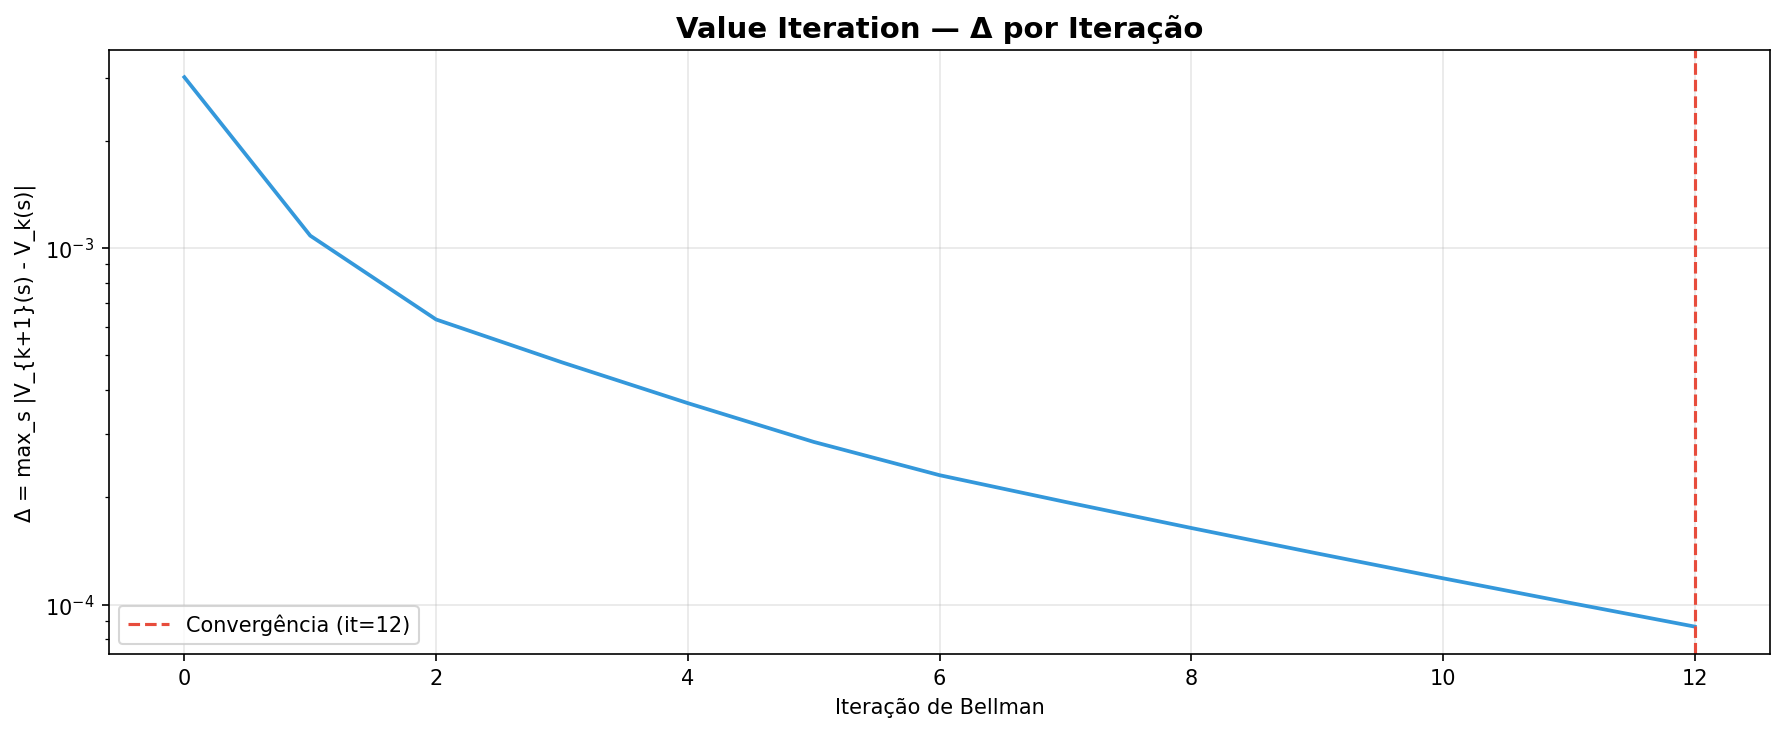
\includegraphics[width=0.75\linewidth]{figures/vi_delta_v2.png}
    \caption{Erro máximo de Bellman ($\Delta$) por iteração do Value Iteration. Escala logarítmica no eixo Y. A linha tracejada vermelha indica a iteração em que $\Delta$ cruza $\theta=10^{-4}$.}
    \label{fig:vi_convergence}
\end{figure}

\subsection{Curvas de Aprendizado}
A Figura~\ref{fig:learning_curves} agrega as curvas de recompensa acumulada (média móvel de 50 episódios) para Q-Learning, separadas por estratégia de decaimento de $\epsilon$ (painel para $\gamma=0.8$). Fica evidente que o decaimento \textbf{constante} apresenta o platô mais baixo e maior variância residual, enquanto \textbf{linear} e \textbf{exponencial} crescem monotonicamente para a mesma região ($\sim$$11$), com o exponencial atingindo o platô mais cedo. Também fica nítido que $\alpha=10^{-1}$ leva a curvas instáveis muito abaixo das demais.

\begin{figure}[H]
    \centering
    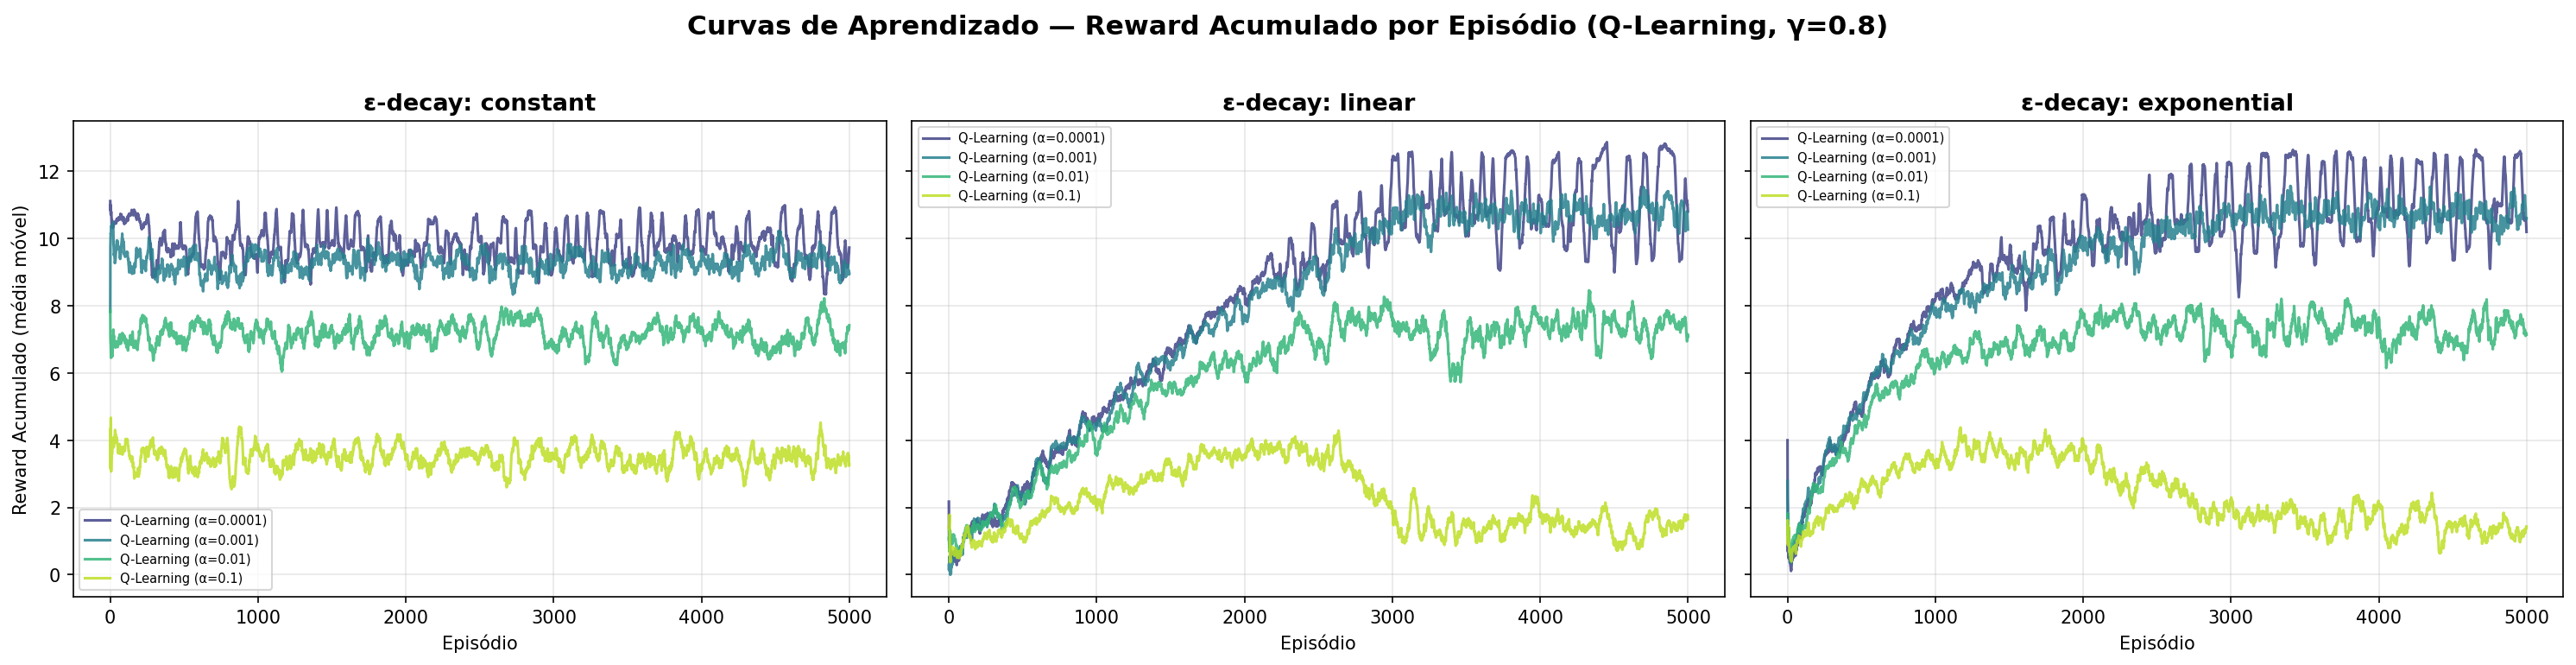
\includegraphics[width=\linewidth]{figures/learning_curves_by_decay_v2.png}
    \caption{Curvas de aprendizado (recompensa acumulada por episódio, média móvel de 50 ep) do Q-Learning, agrupadas por estratégia de decaimento de $\epsilon$ ($\gamma=0.8$). Cada cor corresponde a um valor de $\alpha$.}
    \label{fig:learning_curves}
\end{figure}

\subsection{Estratégia de Exploração}
A Figura~\ref{fig:epsilon_decay} compara as três trajetórias de $\epsilon$ utilizadas. O decaimento exponencial ($\lambda=0.9991$) cai abaixo do piso $\epsilon_{\min}=0.05$ por volta do episódio $3327$, enquanto o linear (parametrizado para decair em $3000$ episódios) atinge o mesmo nível no episódio $3000$. Apesar de o linear terminar antes, o exponencial concentra grande parte da queda nos primeiros $\sim$$1500$ episódios, expondo o agente a $\epsilon$ relativamente baixo (regime de explotação) substancialmente mais cedo — o que explica a diferença de $\sim$$500$ episódios na conquista de 90\% da recompensa final observada na Seção 4.1.

\begin{figure}[H]
    \centering
    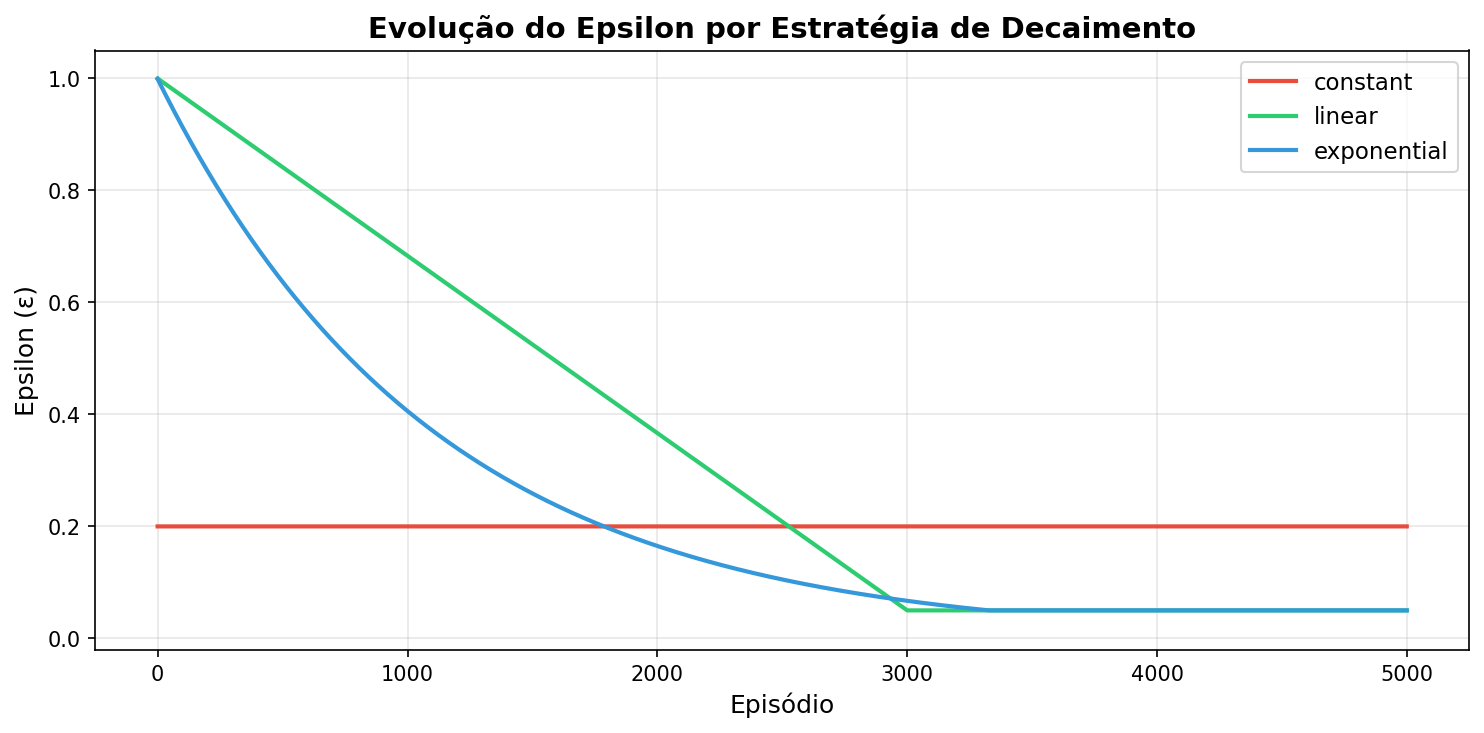
\includegraphics[width=0.65\linewidth]{figures/epsilon_decay_v2.png}
    \caption{Evolução de $\epsilon$ ao longo dos 5000 episódios para as três estratégias avaliadas.}
    \label{fig:epsilon_decay}
\end{figure}

\subsection{Impacto do Fator de Desconto $\gamma$}
A Figura~\ref{fig:gamma_impact} apresenta, à esquerda, as curvas de aprendizado para $\gamma \in \{0.3, 0.5, 0.8, 0.9\}$ no regime de decaimento linear ($\alpha=10^{-4}$) e, à direita, a distribuição de recompensas dos últimos 100 episódios (boxplot) por valor de $\gamma$. A mediana é maximizada em $\gamma=0.3$ ($12.36$) e decai progressivamente até $\gamma=0.9$ ($10.34$), com o desvio padrão crescendo de $0.81$ para $\sim$$2.50$. Esse padrão sinaliza que, neste MDP de log-retornos diários, horizontes longos amplificam variância sem ganho proporcional na recompensa esperada.

\begin{figure}[H]
    \centering
    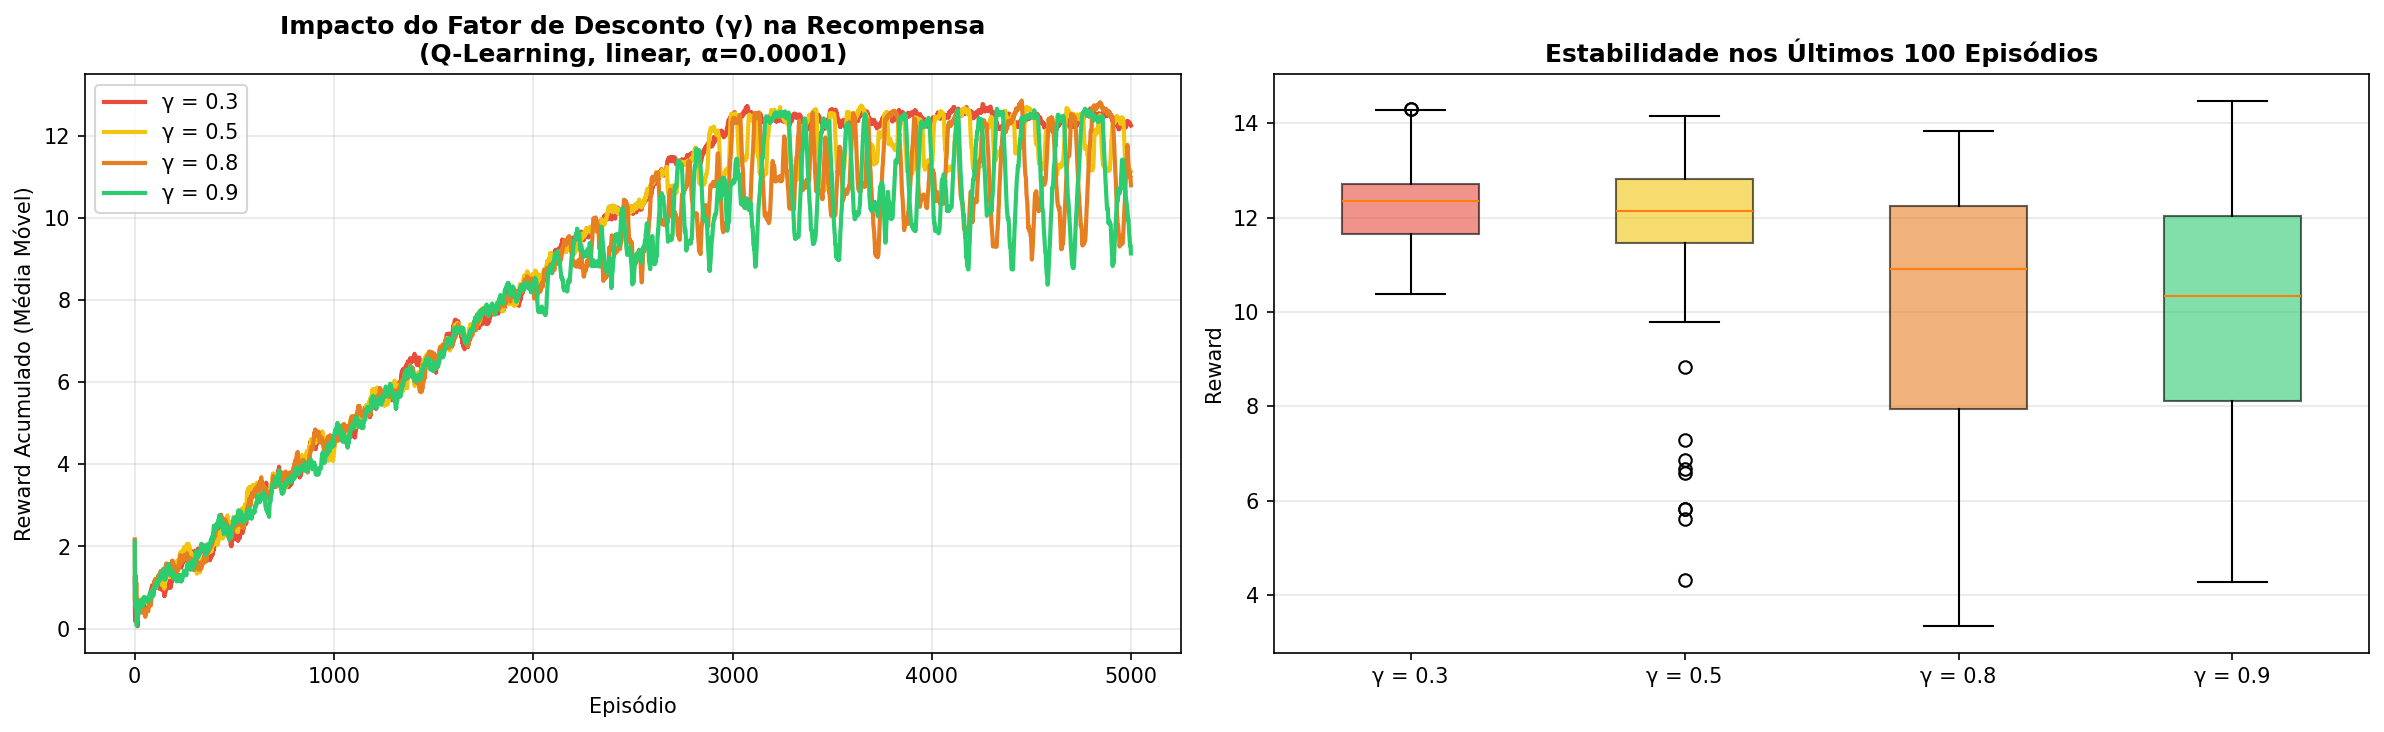
\includegraphics[width=\linewidth]{figures/gamma_impact_v2.png}
    \caption{Esquerda: curvas de aprendizado para diferentes $\gamma$. Direita: distribuição de recompensa nos últimos 100 episódios por $\gamma$.}
    \label{fig:gamma_impact}
\end{figure}

\subsection{Heatmap de Hiperparâmetros}
A Figura~\ref{fig:heatmap} resume, em uma única visualização, a recompensa média dos últimos 100 episódios para todas as combinações de $(\alpha, \text{decay})$ no Q-Learning com $\gamma=0.8$. A coluna $\alpha=10^{-1}$ é uniformemente avermelhada (recompensas entre $\sim$$1.3$ e $\sim$$3.4$), e a região $(\alpha \in [10^{-4}, 10^{-3}],\ \text{decay} \in \{\text{linear, exponencial}\})$ concentra os melhores resultados, com pico em $(\alpha=10^{-4},$ exponencial$)$.

\begin{figure}[H]
    \centering
    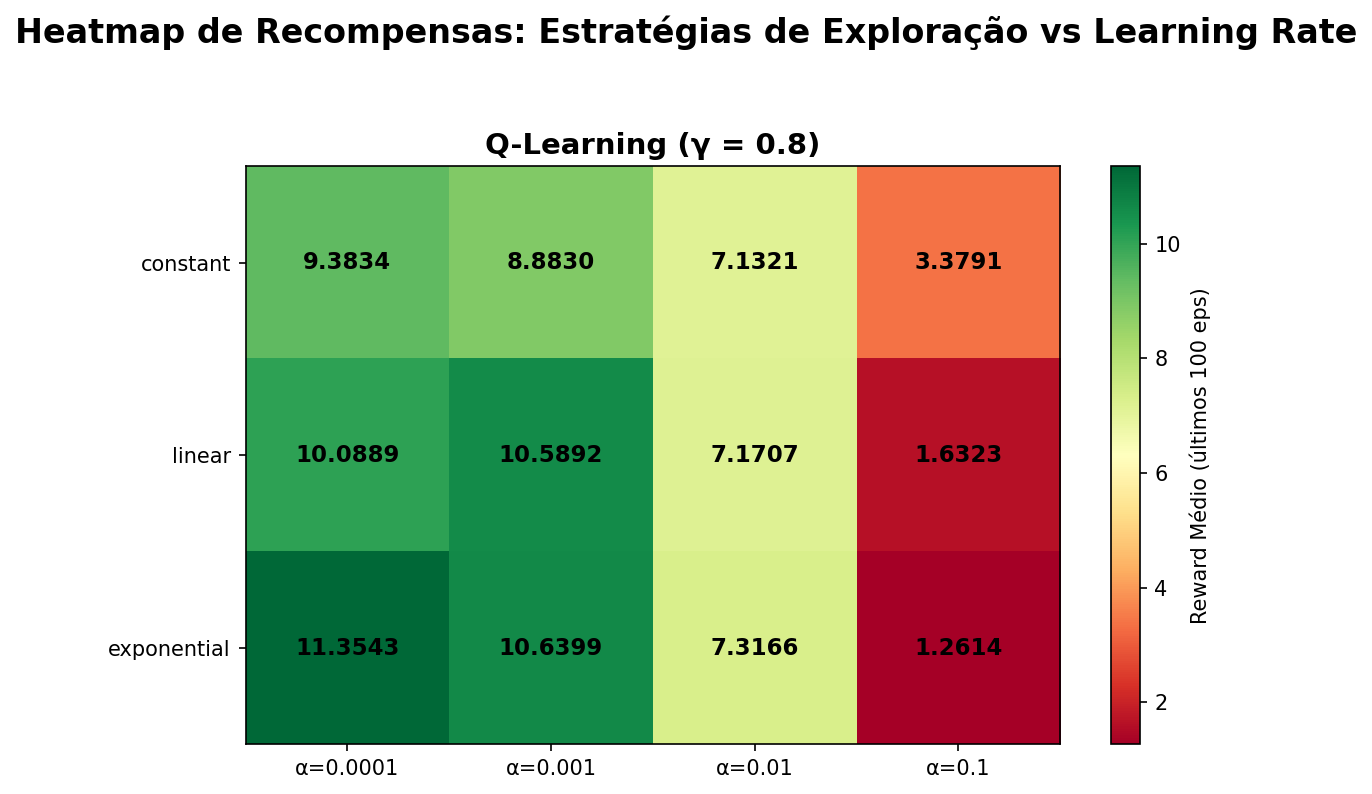
\includegraphics[width=0.7\linewidth]{figures/heatmap_decay_alpha_v2.png}
    \caption{Recompensa média (últimos 100 ep) em função do tipo de decaimento e da taxa de aprendizado para o Q-Learning, com $\gamma=0.8$.}
    \label{fig:heatmap}
\end{figure}

\subsection{Mapa de Valores $V(s)$ e Política Aprendida $\pi(s)$}
A Figura~\ref{fig:value_policy} sintetiza o conhecimento adquirido pelo melhor agente (Q-Learning, decay exponencial, $\alpha=10^{-4}$, $\gamma=0.3$) em formato tabular: à esquerda, $V(s) = \max_a Q(s,a)$; à direita, $\pi(s) = \arg\max_a Q(s,a)$, codificada por cor (verde = comprar, cinza = manter, vermelho = vender). Os 16 estados são organizados em uma grade $4\times4$, indexada pelas duplas $(p, \upsilon)$ nas linhas e $(\mu, \rho)$ nas colunas. A política aprendida diferencia explicitamente entre estados com e sem posição aberta, evidenciando que o agente aprendeu uma regra contextual de entrada e saída em vez de uma heurística trivial baseada apenas em um indicador isolado.

\begin{figure}[H]
    \centering
    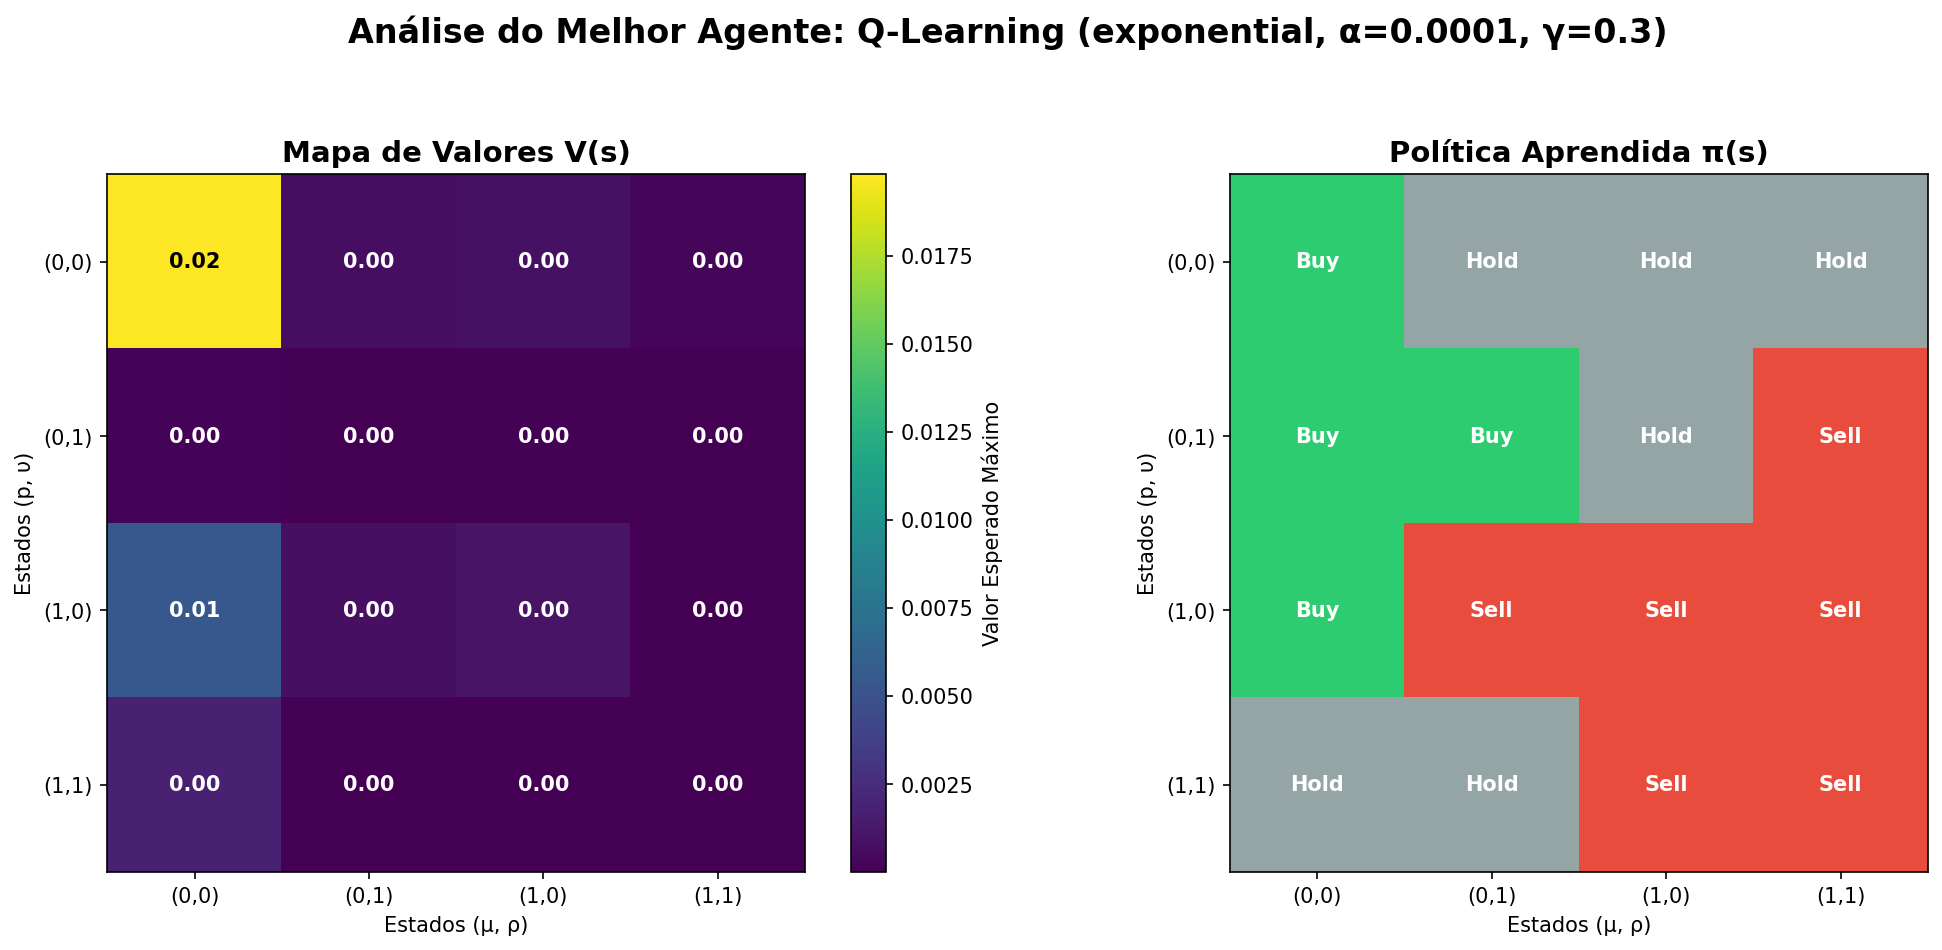
\includegraphics[width=0.95\linewidth]{figures/value_policy_v2.png}
    \caption{Mapa de valores $V(s)$ (esquerda) e política $\pi(s)$ aprendida (direita) do melhor agente. Eixos representam as projeções 2D do estado tetra-dimensional $(p, \upsilon, \mu, \rho)$.}
    \label{fig:value_policy}
\end{figure}

\subsection{Generalização: Treino vs.\ Teste}
A Figura~\ref{fig:train_test} apresenta, à esquerda, a recompensa de treino (média dos últimos 100 episódios) das 10 melhores configurações, com o ponto vermelho destacando o único valor de teste medido — o do melhor agente (Q-Learning exponencial, $\alpha=10^{-4}$, $\gamma=0.3$). À direita, mostra-se o retorno acumulado passo a passo do mesmo agente no conjunto de teste, terminando em $+6.82$. A diferença em valor absoluto entre treino ($\approx 12.52$) e teste ($+6.82$) é parcialmente explicada pelo tamanho do conjunto de teste, que é $\sim$$2{,}33\times$ mais curto que o de treino. Normalizando por \textit{step}, a recompensa por \textit{step} de teste ($3{,}58 \times 10^{-4}$) supera a de treino ($2{,}82 \times 10^{-4}$) — comportamento detalhado em §\ref{sec:limites}.

\begin{figure}[H]
    \centering
    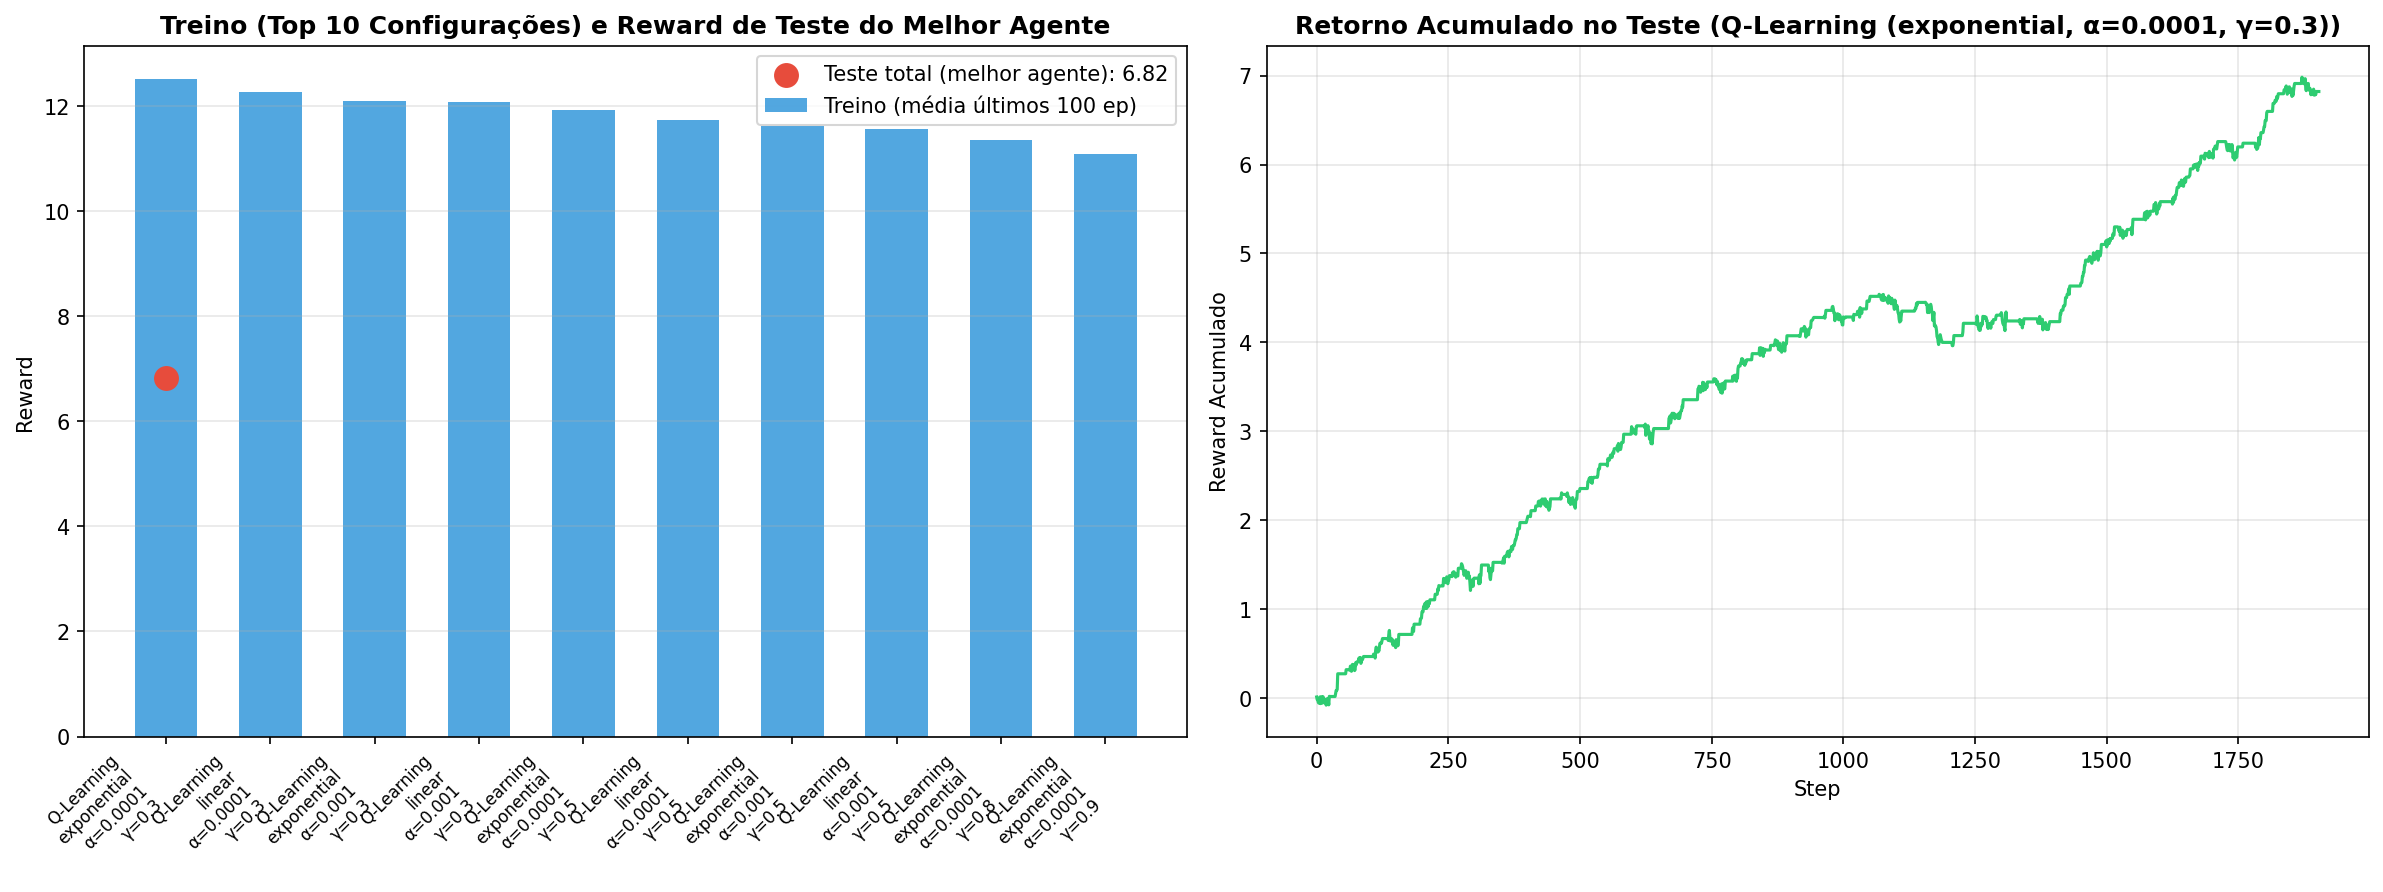
\includegraphics[width=\linewidth]{figures/train_vs_test_v2.png}
    \caption{Esquerda: comparação de recompensa em treino vs.\ teste para as 10 melhores configurações. Direita: retorno acumulado passo a passo no conjunto de teste para o melhor agente.}
    \label{fig:train_test}
\end{figure}

\subsection{Trajetória do Agente}
A Figura~\ref{fig:trajectory} sobrepõe ao preço de fechamento da Amazon (período de teste) as regiões onde a política aprendida mantém posição comprada (verde). A inspeção visual revela que o agente alterna posições \textit{long} e \textit{flat} ao longo de todo o histórico de teste, concentrando posições compradas em segmentos que coincidem com tendências de alta — comportamento consistente com o retorno total positivo ($+6.82$) registrado na Figura~\ref{fig:train_test}.

\begin{figure}[H]
    \centering
    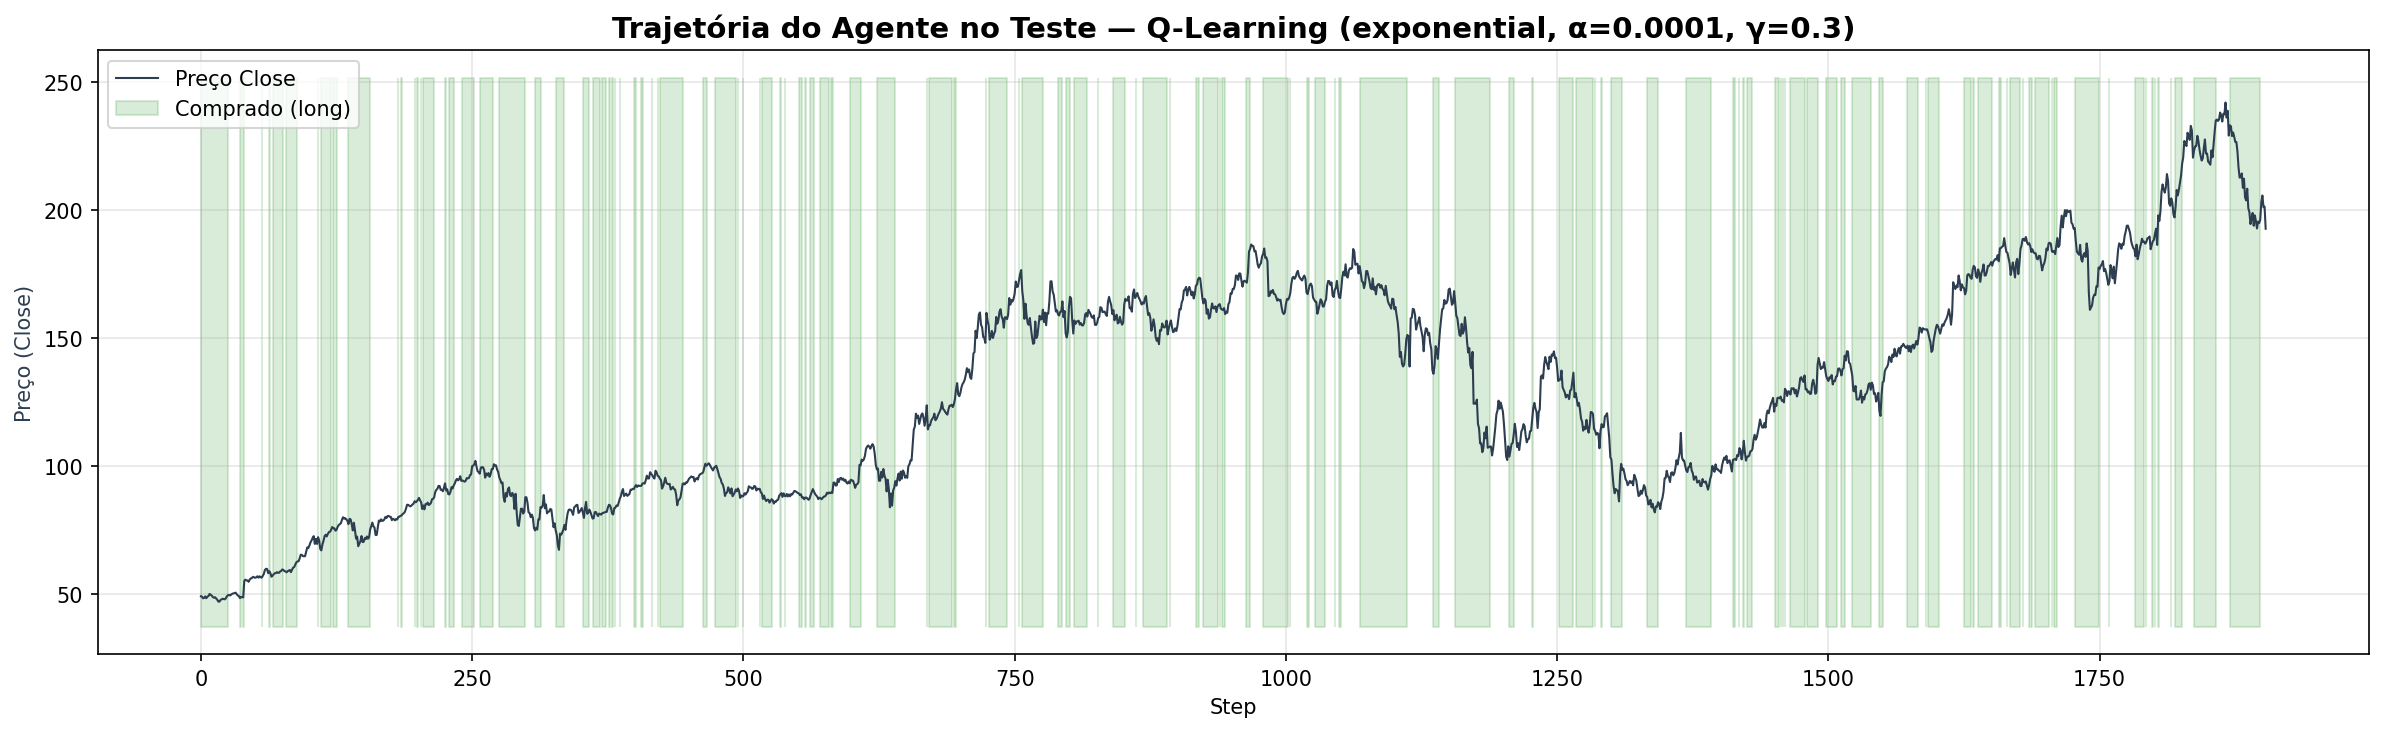
\includegraphics[width=\linewidth]{figures/trajectory_v2.png}
    \caption{Trajetória do melhor agente no conjunto de teste. Linha preta: preço de fechamento; faixas verdes: \textit{steps} em que a posição é \textit{long}.}
    \label{fig:trajectory}
\end{figure}

\section{Discussão}
A aplicação de Aprendizado por Reforço ao contexto do mercado financeiro revelou nuances importantes sobre a modelagem de Processos de Decisão de Markov (MDPs) em ambientes de alta incerteza. A seguir, discutimos os principais desafios, limitações e aprendizados extraídos do projeto.

\subsection{Dificuldades Encontradas}
A principal dificuldade na etapa de modelagem consistiu na formulação do espaço de estados e no \textit{Reward Shaping} (modelagem da recompensa). O mercado financeiro é um ambiente contínuo e ruidoso e discretizar indicadores técnicos (MACD, RSI e Volatilidade) em variáveis binárias exigiu um esforço analítico para garantir que o estado mantivesse representatividade estatística sem causar uma explosão combinatória na Tabela Q.

Além disso, o ajuste do custo de transação ($c$) na função de recompensa provou-se um desafio sensível: valores muito altos faziam o agente adotar uma postura excessivamente passiva (evitando operar para não pagar taxas), enquanto valores muito baixos geravam \textit{overtrading}, onde o agente comprava e vendia a cada flutuação mínima, corroendo o lucro real.

\subsection{Trade-offs Observados}
O treinamento evidenciou o clássico \textit{trade-off} entre estabilidade e velocidade de adaptação, ditado pela taxa de aprendizado ($\alpha$). Taxas menores ($\alpha \le 0.001$) garantiram uma convergência mais segura, mas exigiram milhares de episódios.

Outro \textit{trade-off} central observado é entre o tamanho do fator de desconto $\gamma$ e a estabilidade do aprendizado: valores menores ($\gamma=0.3$) entregaram tanto a maior média de recompensa ($12.26$) quanto o menor desvio padrão ($0.81$), enquanto $\gamma=0.9$ caiu para média $10.03$ e desvio $2.50$. Esse padrão é específico do domínio: como o reward por \textit{step} é o log-retorno diário descontado pelo custo de transação, horizontes longos absorvem mais ruído de mercado sem ganho proporcional, levando o agente a decisões menos consistentes na fase final de treino.

\subsection{Impacto da Exploração}
Os resultados comprovaram que a exploração mal gerenciada degrada a convergência: a estratégia $\epsilon$ constante apresentou recompensa média global $7.38$ contra $7.58$ (exponencial) e $7.32$ (linear) — diferença pequena no agregado, mas com picos notavelmente maiores em linear/exponencial nas melhores configurações. A adoção do decaimento exponencial atingiu 90\% do platô de recompensa cerca de $500$ episódios mais cedo do que o decaimento linear, ao concentrar grande parte da queda de $\epsilon$ nos primeiros $\sim$$1500$ episódios. A Figura~\ref{fig:epsilon_decay}, lida em conjunto com a Figura~\ref{fig:learning_curves}, oferece evidência direta dessa dinâmica: o platô de recompensa coincide visualmente com o trecho em que $\epsilon$ atinge $\epsilon_{\min}$, confirmando que estabilização da política e silenciamento da exploração são fenômenos acoplados.

\subsection{Limitações do Modelo}\label{sec:limites}
A diferença entre o retorno acumulado de treino ($\approx 12.52$ na melhor configuração) e o de teste ($+6.82$ no mesmo agente avaliado em modo \textit{greedy}) merece análise cuidadosa: o conjunto de teste é cerca de $2{,}33\times$ mais curto do que o de treino (1904 \textit{steps} vs.\ 4442), o que deflaciona naturalmente o retorno cumulativo. Ao normalizar por \textit{step}, o agente entrega $3{,}58 \times 10^{-4}$ de log-retorno por dia no teste contra $2{,}82 \times 10^{-4}$ por dia no treino — ou seja, o agente é cerca de $27\%$ \textit{mais} eficiente no conjunto de teste do que no de treino. Esse resultado descarta a hipótese de simples \textit{overfitting} ao regime de \textit{noise injection} (perturbação multiplicativa de $\pm 5\%$) e sugere que a política generaliza bem para a série bruta. Ainda assim, o uso de uma única trajetória de teste (sem perturbações) limita a inferência estatística sobre robustez fora da amostra. Para além desse aspecto, persistem limitações inerentes à formulação tabular adotada:
\begin{itemize}
    \item \textbf{Perda de Magnitude:} Ao binarizar o RSI e o MACD, o agente sabe se o mercado está "sobrecomprado" ou "sobrevendido", mas perde a noção da \textit{força} (magnitude contínua) desse movimento.
    \item \textbf{Não-Estacionariedade:} MDPs assumem que a probabilidade de transição $T(s, a, s')$ é estacionária. No entanto, o mercado financeiro real muda suas dinâmicas ao longo do tempo (devido a fatores macroeconômicos não observáveis pelo agente).
    \item \textbf{Ações Restritas:} O modelo não permite \textit{short-selling} (venda a descoberto) nem o fracionamento de aportes, limitando a alocação de risco.
\end{itemize}

\subsection{Relação entre Teoria e Prática}
A teoria estabelece que o \textit{Value Iteration} converge para a política ótima de forma exata caso o modelo $T(s, a, s')$ seja conhecido. Na prática, demonstrou-se que é possível contornar a ausência desse modelo construindo uma matriz empírica de transições a partir do histórico de dados.

A Figura~\ref{fig:value_policy} torna explícita a estrutura aprendida: a política não recai sobre uma regra única e simples (como "comprar quando MACD positivo"), mas combina os indicadores de forma contextual, com decisões diferentes para o agente posicionado ($p=1$) e flat ($p=0$) — comportamento típico de uma política estado-condicional aprendida por TD em vez de uma regra heurística fixa.

Contudo, a prática também revelou a flexibilidade dos métodos \textit{Model-Free} (\textit{TD Learning}) para este tipo de problema. O Q-Learning provou ser adaptável à natureza estocástica das ações da Amazon, aprendendo puramente por tentativa e erro sem sofrer \textit{overfitting} a uma matriz de transição estática. O projeto consolida a teoria de que, para problemas onde o ambiente é uma "caixa preta" ruidosa, métodos baseados em amostragem temporal são ferramentas mais robustas e generalizáveis do que o planejamento clássico — ainda que o \textit{Value Iteration} mantenha a vantagem de uma convergência drasticamente mais barata em iterações ($12$ varreduras contra $5000$ episódios).

\end{document}
